\chapter{Lecture four: Behaviour}
\section{Behaviour}

\subsection{Result}
The result of this activity is a schematic of behavioural paths.

\begin{figure}[H]
    \centering
    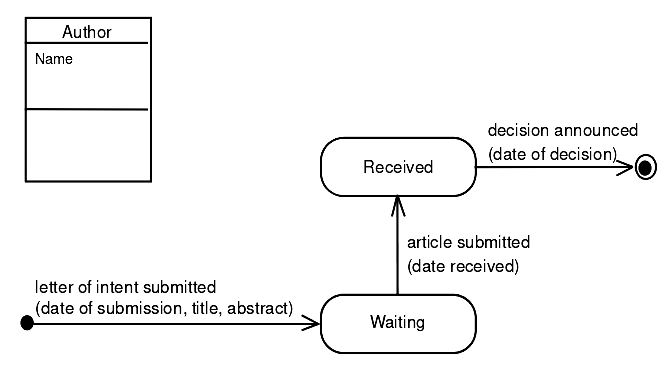
\includegraphics[width=.6\textwidth]{figures/behaviourresult.png}
\end{figure}

\subsection{Activities}

The behaviour activity includes four activities. Start with event table and class diagram. We start with describing behavioural patterns for each class, using related events. General patterns of class behaviour are used to improve description and discover new ways of expressing aspects of the PD. These activities unveil weakness in the structure, and will generate ideas for new structure and classes. Activity ends with specification of main attributes for all classes and events.
\begin{figure}[H]
    \centering
    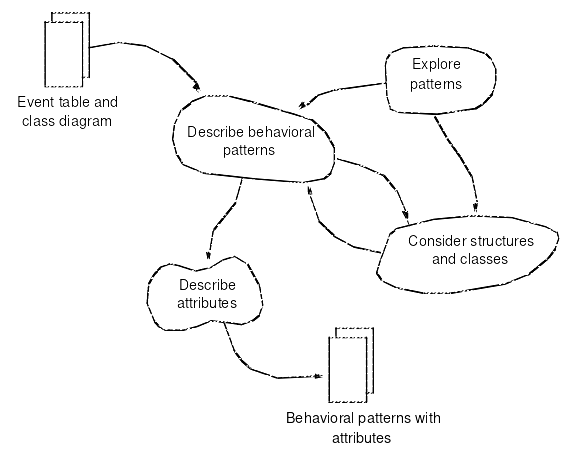
\includegraphics[width=0.65\textwidth]{figures/behaviouractivities.png}
\end{figure}

\subsection{Key concepts}
\subsubsection{Event Traces}
Event trace: A sequence of events involving a specific object. A customer object in figure \ref{fig:behaviouralpattern} might have following event trace: account opened - amount deposited - amount withdrawn - amount deposited - account closed. 

\subsubsection{Behavioural pattern}
For practical reasons, groups of objects are described instead of describing behaviour of every object. For the same reasons, the behaviour of every object is not described, instead we describe a behavioural pattern for object classes. \newline \textbf{Behavioural pattern:} A description of possible event traces for all objects in a class. 
The behavioural pattern describes behaviour common to all objects of the class. 

\begin{figure}[h]\label{fig:behaviouralpattern}
    \centering
    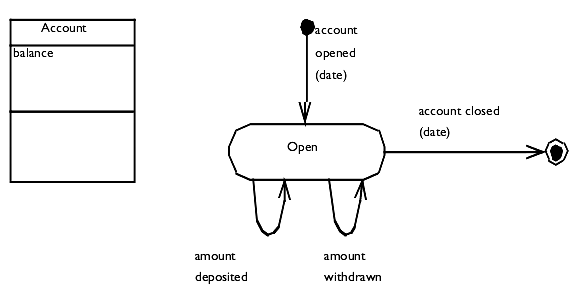
\includegraphics[width=0.6\textwidth]{figures/behaviouralpattern.png}
\end{figure}

\subsubsection{Describe behavioural patterns}
Make event traces for each class. For each of these classes, ask the following:

\begin{itemize}
    \item Which event(s) cause the creation of a problem-domain object? \newline These events are grouped as selections that can cause the creation of an object.
    \item Which event(s) cause the disappearance of a problem-domain object? \newline These events are grouped as selections that can cause the death of an object.
\end{itemize}

\noindent Typical event traces can be found with the following questions:
\begin{itemize}
    \item Which events occur together in a sequence?
    \item Are there any alternative events?
    \item Can a given event occur more than once?
    \item Is the overall form structured or unstructured?
\end{itemize}


\subsubsection{Control structures}

A behavioural patterns orders individual events in time using control structures:

\begin{itemize}
    \item \textit{Sequence:} Events in a set occur one by one. Denoted using "+"
    \item \textit{Selection:} Exactly one out of a set of events occurs. Denoted using "l"
    \item \textit{Iteration:} An event occurs zero or more times. Denoted using "*"
\end{itemize}

A behavioural pattern with these can be described with a regular expression. For example: account opened + (amount deposited | amount withdrawn)* + account closed.

A statechart diagram has the same expressive capability as the regular expression, and these are drawn as such:

\begin{figure}[H]
    \centering
    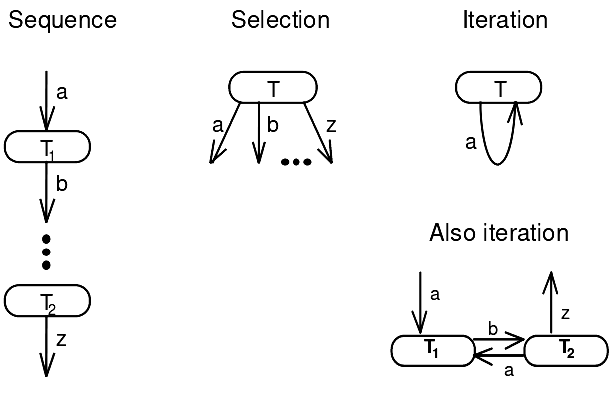
\includegraphics[width=.5\textwidth]{figures/behaviouralcontrol.png}
\end{figure}

\subsection{Modelling techniques}
\subsubsection{From event traces to behavioural patterns}
\begin{figure}[H]
    \centering
    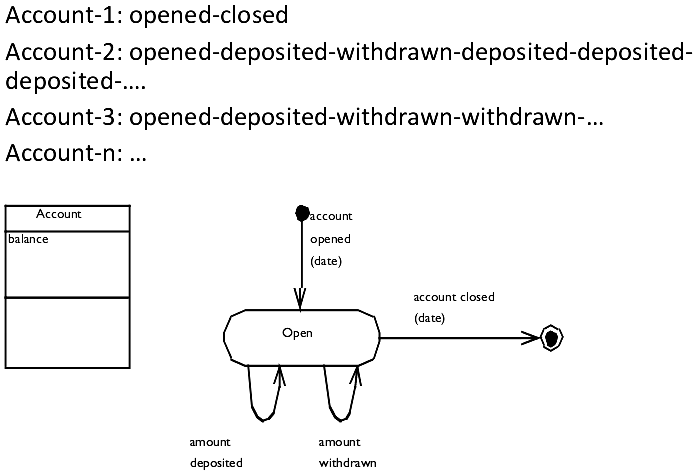
\includegraphics[width=.75\textwidth]{figures/eventtracetobehaviouralpattern.png}
\end{figure}

It's clear that all event traces can be represented through the actions of the behavioural pattern. 

\subsubsection{Conditions in statechart diagrams}
Typically the transition in a statechart diagram occurs as a result of problem-domain events. In special cases you may want to supplement with another form of transition - one that occurs when a stated condition is true. 

The requirement is stated in the square brackets in the figure. This conditional transition is useful both with administrative and technical systems.

\begin{figure}[H]
    \centering
    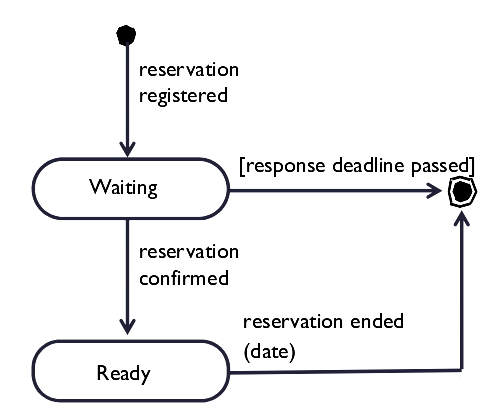
\includegraphics[width=.4\textwidth]{figures/conditionalstatechart.png}
\end{figure}

\subsubsection{Common events}
It's useful to create behavioural patterns for common events, as these are naturally the most abundant in the system to be designed.

\subsubsection{Consider structures}
Aggregation and association:
\begin{itemize}
    \item If two or more objects have common events, consider adding an aggregation or association structure between them.
    \item If two classes are related by an aggregation or association structure, at least one common event should be considered.
\end{itemize}
\noindent Generalisation:
\begin{itemize}
    \item If the same event is tied to two classes, consider whether one class is a generalisation of the other.
\end{itemize}

\subsubsection{Hierarchical states}
Consider using this pattern to simplify modelling.

\begin{figure}[H]
    \centering
    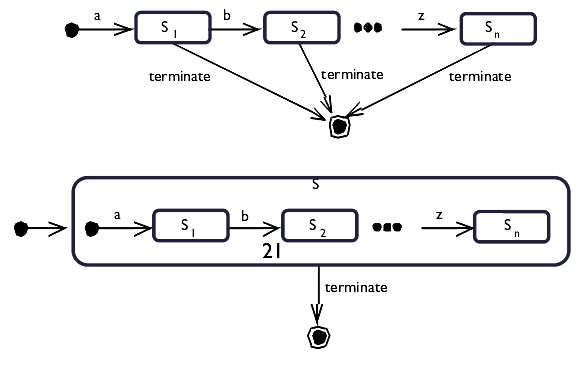
\includegraphics[width=.65\textwidth]{figures/hierarchicalstate.png}
\end{figure}

\subsubsection{Describe attributes}
The following questions can be asked to describe attributes. Class attributes:
\begin{itemize}
    \item What are the general characteristics of the class?
    \item What basic data must be captured about the objects from this class?
    \item What results from an event trace must be captured?
\end{itemize}

\noindent Event attributes:
\begin{itemize}
    \item What time did the event occur?
    \item Which amount did it concern?
\end{itemize}


\subsection{Summary}
\begin{figure}[H]
    \centering
    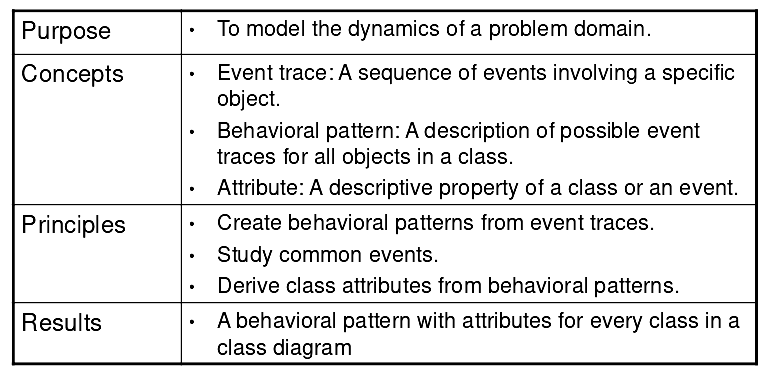
\includegraphics[width=.7\textwidth]{figures/behavioursummary.png}
\end{figure}

\section{Example on streaming}\label{behaviour:streamingservice}
Recall the FACTOR-description and class diagram from section \ref{structure:streamingservice} on a streaming service. Following are three statechart diagrams for Customer, watched, and Movie:

\begin{figure}[H]
    \centering
    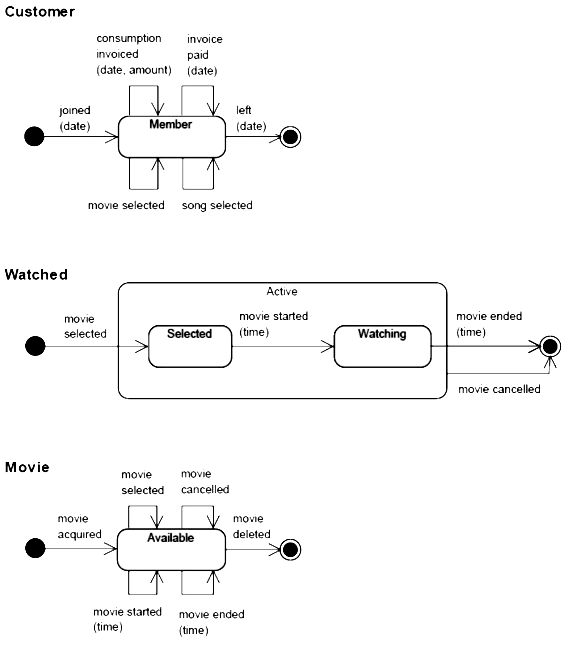
\includegraphics[width=.6\textwidth]{figures/statechartstreaming.png}
\end{figure}

\section{Explore patterns}
We'll focus on three basic behaviour patterns. These can be used to improve an outline or contribute to a completely new idea for part of the problem-domain model.

\subsection{Stepwise relation pattern}
\begin{figure}[H]
    \centering
    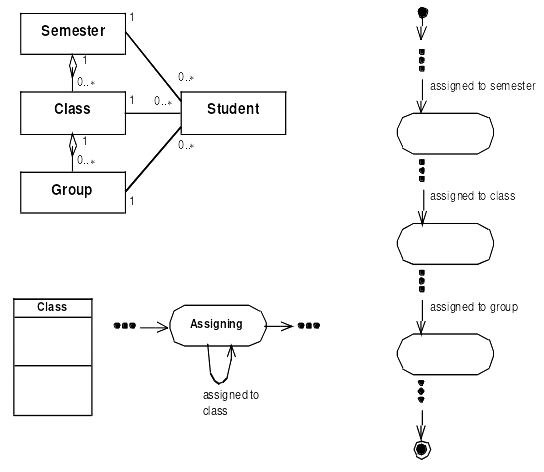
\includegraphics[width=.6\textwidth]{figures/stepwiserelation.png}
\end{figure}

This pattern is used when the elements of a hierarchy  resembles a stepwise or sequential manner. The figure shows a situation where students are first assigned a semester, then a class, and lastly a group. The group is an element of a class, the class is an element of a semester.

\subsection{Stepwise role pattern}
\begin{figure}[H]
    \centering
    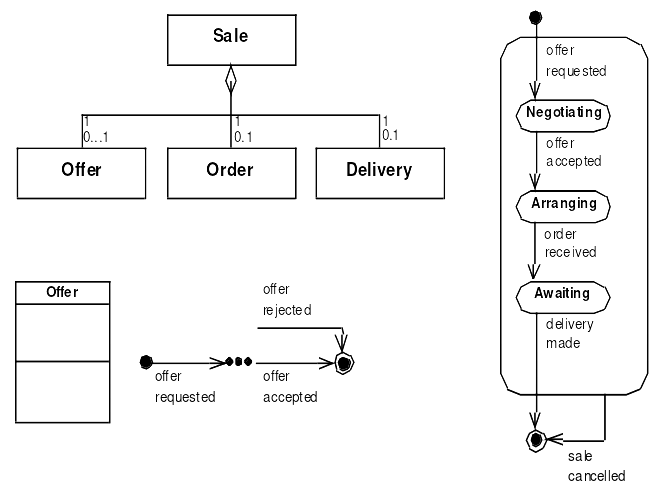
\includegraphics[width=.6\textwidth]{figures/stepwiserole.png}
\end{figure}

This pattern is used to describe interaction between several objects over time, but more-so on the horizontal dimension in a class diagram than the vertical dimension.
The figure shows a sale modelled as consisting of an offer, an order, and a delivery. The statechart diagrams show how these objects interact and gets created. E.g. an offer is created when it is requested, and terminates when the offer is accepted or rejected. The two other subobjects behave similarly.
A sale can be terminated at any time in the course of its life, as shown by \texttt{sale cancelled}.

Note that this pattern is simple when the order is sequential. As soon as the parts become interwoven and mutually dependent the complexity of the diagram increases rapidly.
\subsection{Composite pattern}
\begin{figure}[H]
    \centering
    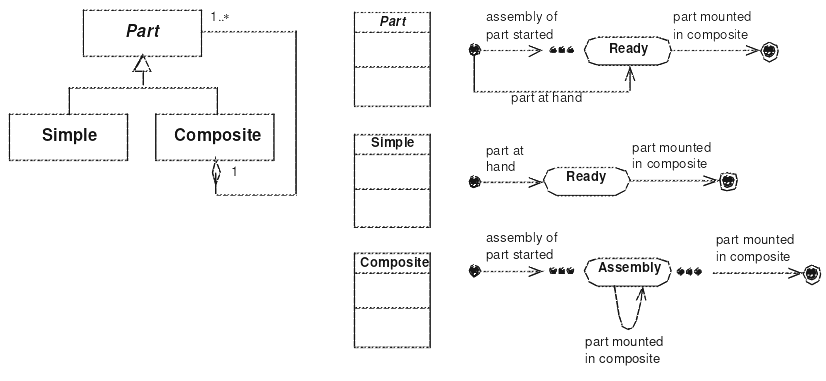
\includegraphics[width=.8\textwidth]{figures/compositepattern.png}
\end{figure}

This pattern offers a way to describe the creation and destruction of a hierarchy using a detailed structure that is unknown at model-development time. 
The figure shows an example, where \texttt{Part} is an abstract class, and \texttt{Simple} and \texttt{Composite} are specialisations. A composite part aggregates several parts, where each part is one of the two specialisations.

The figure also shows the behavioural patterns for the tree classes. A parts statechart diagram imposes limits on specialisations. A simple part is immediately ready, as it does not need assembly. If this simple part is mounted in a enclosing composite its separate life ends and it continues to live on only as an integrated part of a composite. Likewise, if the composite is mounted, with all it subparts, on another composite, its life is terminated and it continues on as a part of a new composite.

The key point in this pattern is that the top-level behaviour requires some behaviour from the level beneath it, which in turn requires behaviour from the level beneath it, and so on. This ends up being a recursive description. 

\section{Conceptually; class, event, or attribute?}
We have some information from the problem domain, e.g., a customer buys a chair for 100 DKK. How can this be modelled?

\begin{itemize}
    \item \textbf{Attribute:} In the Customer class we introduce an attribute \texttt{bought} which is increased by the amount that the customer has bought for.
    \item \textbf{Event:} For the Customer class we introduce a \texttt{bought} event with the price of the chair as an attribute. This allows us to produce a list of the amounts the user has purchased for.
    \item \textbf{Class/Object:} We introduce a \texttt{Bought} class that is aggregated by the Customer class, it aggregates an object of the Product class and has some events. This allows us to model events for and behavioural structure on \texttt{Bought} objects.
\end{itemize}

\section{Principles}
\subsection{Create behavioural patterns from event traces}
The problem-domain dynamics are described by behavioural patterns for each class in the model. The behavioural pattern describes legal event traces and thereby determines the order of events for each object in the class.

\subsection{Study common events}
Common events point out important, dynamic relations in the model. common events can cause reconsideration of the choice of classes and their structural relations.

\subsection{Derive class attributes from behavioural patterns}
The attributes necessary for capturing relevant data about objects and events are derived from the class definition and the behavioural pattern.

\section{Challenges in this activity}
\begin{itemize}
    \item Start with event traces for the simple classes
    \item Describe behavioural patterns from the event traces
    \item Continue with the more complex classes
    \item If the behavioural pattern becomes too complicated, consider using the stepwise role or stepwise relation pattern - \textit{this introduces new classes}
    \item Make sure there are behavioural patterns that control sequence and some that don't (structured/unstructured)
    \item Add attributes to classes and events
    \item Check the behavioural patterns against the class diagram
\end{itemize}